\documentclass[12pt]{article}
\usepackage[utf8]{inputenc}

\usepackage[margin = 0.7in]{geometry}
\usepackage{amsmath}
\usepackage{amsfonts}
\usepackage{amssymb}
\usepackage{amsthm}
\usepackage{graphicx}
\usepackage{placeins}
\usepackage{enumitem}
\usepackage{dsfont}

\newcommand{\N}{\mathbb{N}}
\newcommand{\Z}{\mathbb{Z}}
\newcommand{\R}{\mathbb{R}}
\newcommand{\E}{\mathbb{E}}
\newcommand{\Q}{\mathbb{Q}}
\newcommand{\de}{\mathrm{d}}
\newcommand{\one}{\mathds{1}}

\title{ECON 899: Problem Set 1}
\author{Katherine Kwok}
\date{September 2021}

\begin{document}

\maketitle
\noindent \textbf{Overview: } For this assignment, the goal is to add uncertainty over technology shocks to a dynamic programming problem in an infinite horizon growth model. In particular, we are asked to modify existing matlab \textit{or} julia code, and fortran code. I have written up the code in julia, fortran, and a parallelized verion of the julia code. \\\\
\textbf{Dynamic Programming Problem: } The dynamic programming problem is as follows
\begin{align*}
    V(k, z) &= \max_{k'} \log(c) + \beta \sum_{z' \in Z} \pi(z'|z) V(k', z') \\
    \text{s.t. } k' &= (1-\delta)k + zk^{\theta} - c
\end{align*}
where $z \in Z = \{Z^g, Z^b\}$, and $\pi(z'|z)$ is a given cell in the transition matrix 
\begin{align*}
    \Pi &= \begin{pmatrix} 0.977 & 0.023 \\ 0.074 & 0.926\end{pmatrix}
\end{align*}
We are also given the parameters $\theta = 0.36, \delta = 0.025, \beta = 0.99$.\\\\
\textbf{Value Function: }Using julia and fortran, we can compute the value and policy functions that solve the problem. I find that the value function is increasing over $k$ and concave. The plots of the value functions in both good states and bad states are below.
\begin{figure} [!htbp]
    \centering
    \begin{minipage}{0.45\textwidth}
        \centering
        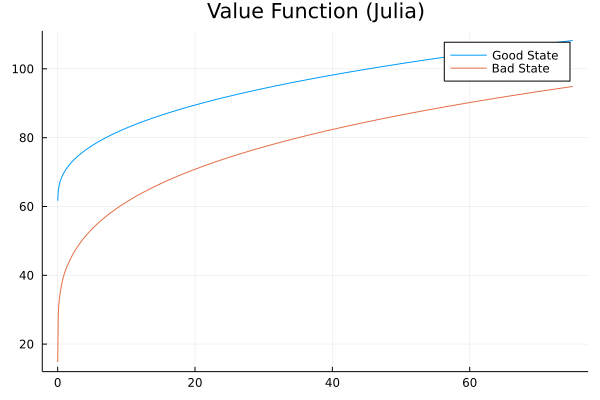
\includegraphics[width=\textwidth]{02_Value_Functions.png}
        \caption{Value Function from Julia Code}
    \end{minipage}\hfill
    \begin{minipage}{0.45\textwidth}
        \centering
        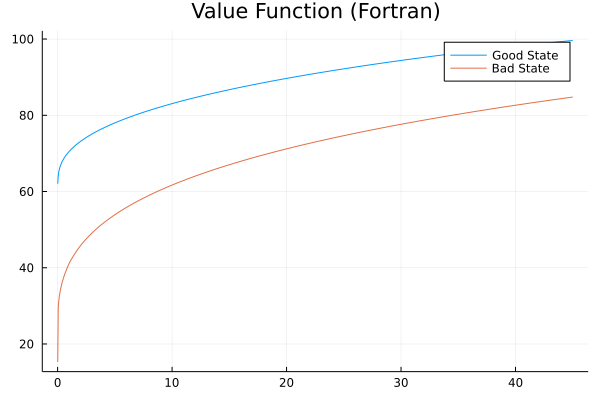
\includegraphics[width=\textwidth]{02_Value_Functions_Fortran.png} 
        \caption{Value Function from Fortran Code}
    \end{minipage}
\end{figure}

\newpage
\noindent \textbf{Policy Function and Savings: } I have plotted the policy functions and the changes in the policy functions for both good and bad states below. Observing the plots below, we see that the policy function is increasing over $k$ and $z$. The policy function slopes upwards, and the function for the good state is higher than that of the bad state. \\\\
To see how savings are affected by $k$ and $z$, we plot the changes in the policy functions, i.e. $k'(k, z) - k$ across $k$ for each possible state $z$. In the bad state, savings decrease as $k$ increases. In the good state, savings initially increases with $k$, but curves downwards eventually. 

\begin{figure} [!htbp]
    \centering
    \begin{minipage}{0.45\textwidth}
        \centering
        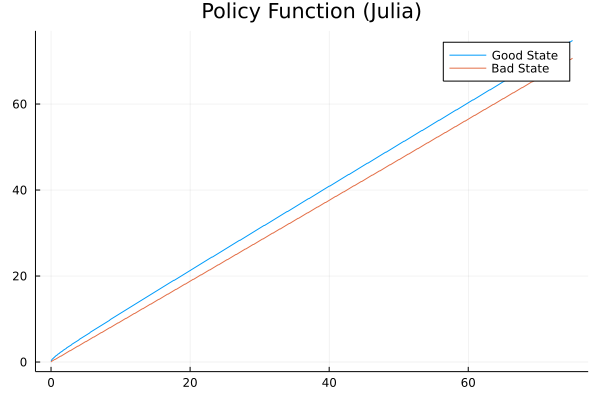
\includegraphics[width=\textwidth]{02_Policy_Functions.png}
        \caption{Policy Function from Julia Code}
    \end{minipage}\hfill
    \begin{minipage}{0.45\textwidth}
        \centering
        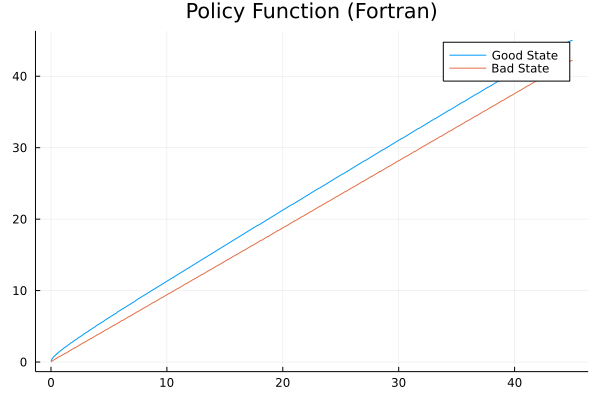
\includegraphics[width=\textwidth]{02_Policy_Functions_Fortran.png} 
        \caption{Policy Function from Fortran Code}
    \end{minipage}
\end{figure}

\begin{figure} [!htbp]
    \centering
    \begin{minipage}{0.45\textwidth}
        \centering
        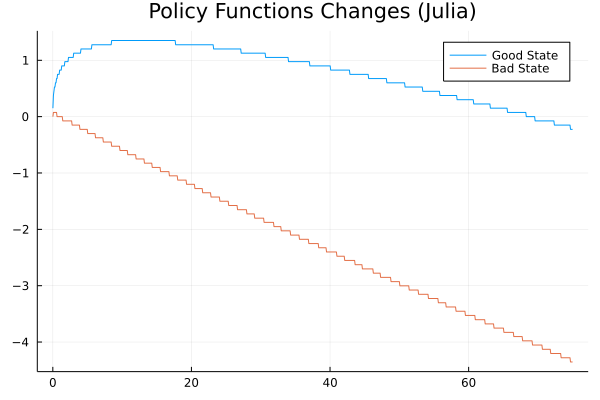
\includegraphics[width=\textwidth]{02_Policy_Functions_Changes.png}
        \caption{Policy Func. Changes from Julia}
    \end{minipage}\hfill
    \begin{minipage}{0.45\textwidth}
        \centering
        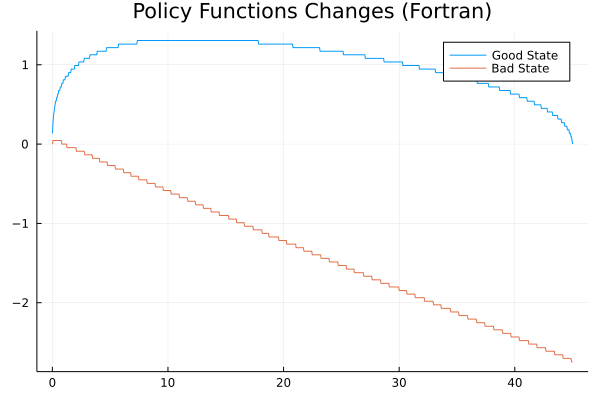
\includegraphics[width=\textwidth]{02_Policy_Functions_Changes_Fortran.png} 
        \caption{Policy Func. Changes from Fortran}
    \end{minipage}
\end{figure}

\newpage
\noindent\textbf{Comparison of Computation Time: } In addition to visualizing the results, we also compare the efficiency of different codes (julia, fortran, and julia parallelized). I ran all codes on my laptop, which has 4 cores. The table below summarizes the computation times:

\begin{table}[!htbp]
    \centering
    \begin{tabular}{c|c|c}
         Julia & Julia (Parallelized) & Fortran \\
         \hline
         6.443 seconds &  6.355 seconds & 13.648 seconds
    \end{tabular}
\end{table}
\noindent As shown above, the parallelized version of julia solves the dynamic programming program the quickest out of the three. All julia and fortran codes are attached with this assignment. 

\end{document}

